% =====================================================================
%  BLOCCO 2 --- Rumore e sensibilità
% =====================================================================

\section{Blocco 2 --- Rumore e NEP}

% --- Slide: modello di rumore ---
\begin{frame}
\frametitle{Modello di rumore --- Blocco~2}

Il segnale misurato \`e affetto da un \textbg{rumore gaussiano generico}
che modella tutti i contributi (Johnson, amplificatore, ADC, \ldots):

\[
  \Delta V_\text{noisy} = \Delta V + \varepsilon, \qquad
  \varepsilon \sim \mathcal{N}(0,\, V_\text{noise}^2)
\]

con $V_\text{noise} = \SI{1e-5}{\volt}$ (floor di rumore totale).

\vspace{0.4em}
\begin{columns}[T]
  \begin{column}{0.48\textwidth}
    \textbf{Rapporto segnale-rumore:}
    \[
      \mathrm{SNR} = \frac{|\Delta V|}{V_\text{noise}}
    \]
    \begin{itemize}
      \item $\mathrm{SNR} \geq 1$: segnale \textbg{ricostruibile}
      \item $\mathrm{SNR} < 1$: \textbr{dominato dal rumore}
    \end{itemize}
  \end{column}
  \begin{column}{0.48\textwidth}
    \textbf{Potenza equivalente di rumore (NEP):}
    \[
      \mathrm{NEP} = \frac{V_\text{noise}}{S}
                   = \frac{V_\text{noise}\,G}{I_\text{bias}\,R_0\,\alpha}
    \]
    Con i parametri nominali:
    \[
      \mathrm{NEP} \approx \SI{2.56e-6}{\watt}
    \]
  \end{column}
\end{columns}

\end{frame}

% --- Slide: tre regimi operativi ---
\begin{frame}
\frametitle{Tre regimi operativi}

\begin{columns}[T]
  \begin{column}{0.33\textwidth}
    \centering
    \textbr{\textbf{Rumore dominante}}\\[0.3em]
    $P < \mathrm{NEP}$\\[0.2em]
    $\mathrm{SNR} < 1$\\[0.2em]
    Il segnale \`e sepolto nel rumore. La misura non \`e affidabile.
  \end{column}
  \begin{column}{0.33\textwidth}
    \centering
    \textbg{\textbf{Ricostruibile}}\\[0.3em]
    $\mathrm{NEP} \leq P < P_\text{sat}$\\[0.2em]
    $\mathrm{SNR} \geq 1$\\[0.2em]
    Il bolometro opera linearmente. $P$ \`e stimabile da $\Delta V$.
  \end{column}
  \begin{column}{0.30\textwidth}
    \centering
    \textcolor{orange}{\textbf{Saturato}}\\[0.3em]
    $P \geq P_\text{sat}$\\[0.2em]
    $|\Delta V| = V_\text{sat}$\\[0.2em]
    L'uscita \`e bloccata a $\pm\SI{1}{\volt}$. Solo un lower bound su $P$.
  \end{column}
\end{columns}

\vspace{0.6em}
\begin{alertblock}{Dinamica del bolometro}
  Il \textbf{range dinamico} utile \`e
  $[\mathrm{NEP},\, P_\text{sat}] =
  [\SI{2.56e-6}{\watt},\; \SI{5e-3}{\watt}]$,
  ovvero circa \textbg{3 decadi} in potenza.
\end{alertblock}

\end{frame}

% --- Slide: grafico blocchi 1-2 ---
\begin{frame}
\frametitle{Grafici --- Modello diretto e rumore}

\begin{center}
  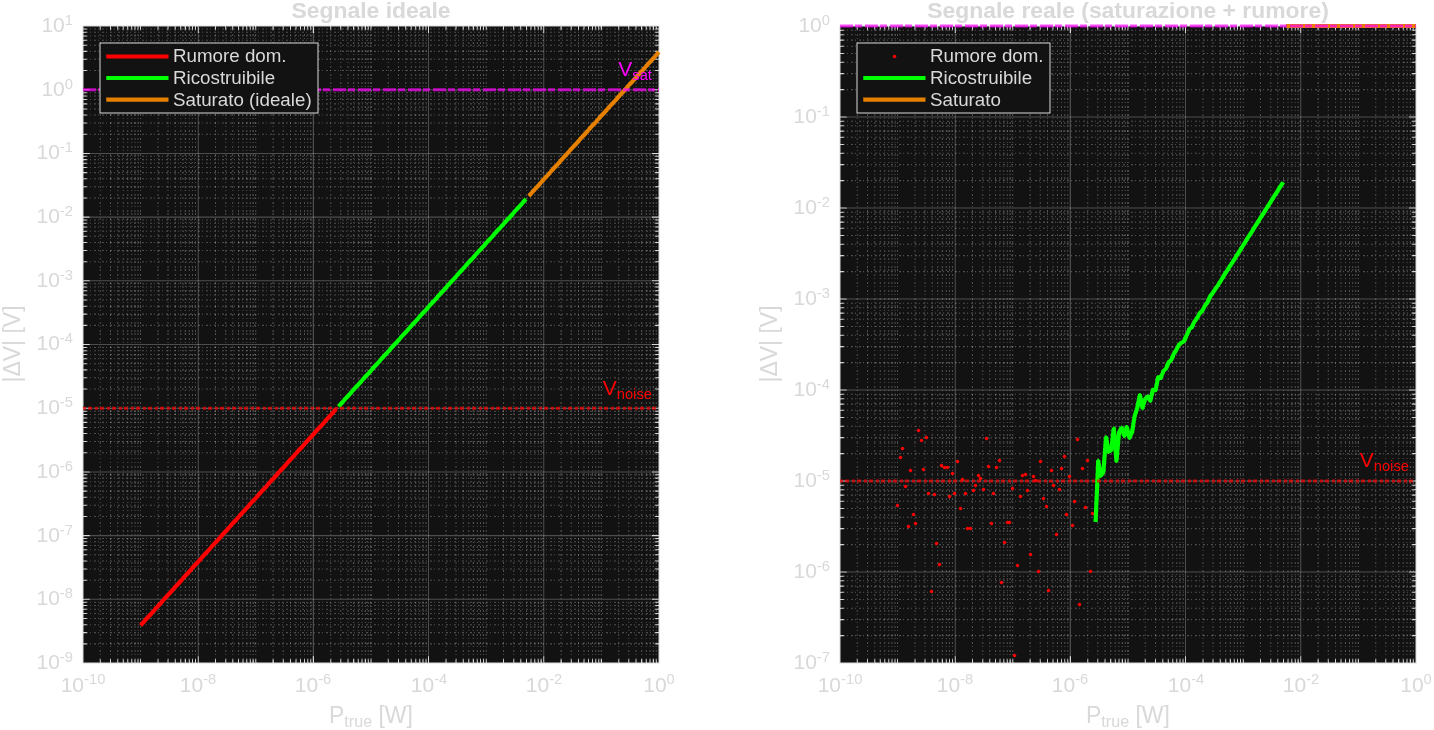
\includegraphics[width=0.90\textwidth]{blocchi_1_2_risultati.png}
\end{center}

\vspace{-0.3em}
\small
\textit{Sinistra}: segnale ideale $|\Delta V_\text{ideal}|$ vs $P$.
\textit{Destra}: segnale reale con saturazione e rumore gaussiano.
I colori indicano il regime: \textbr{rosso} = rumore dominante,
\textbg{verde} = ricostruibile, \textcolor{orange}{arancio} = saturato.

\end{frame}
